\section{随机路径的数值模拟}
\label{sec:ctsp-numerical}

除了少数线性模型，随机微分方程没有显式解，需要在计算机上生成近似路径。本节研究一个已经给定的连续时间模型怎样离散：扩散部分按时间步进，跳跃部分按事件或网格处理，误差则按两种不同的目标衡量——近似路径是否贴近真实路径，近似分布的期望是否贴近真实期望。这里的模型是给定的，任务是忠实地模拟它；下一节反过来设计一个过程去采样给定的目标分布，两类任务的误差含义不同。

\subsection{扩散方程的时间步进}
\label{sec:ctsp-time-stepping}

\paragraph{Euler--Maruyama方法}
第~\ref{chap:ordinary-differential-equations}章的显式Euler方法在每一步冻结左端点的变化率。随机方程沿用同一想法：在每个小区间上把漂移与扩散系数冻结在左端点。取步长$h$、网格$t_k=kh$，令$\widehat{\bm X}_0=\bm X_0$，
\begin{equation}
  \widehat{\bm X}_{k+1}=\widehat{\bm X}_k+\bm b(t_k,\widehat{\bm X}_k)\,h+\bm\sigma(t_k,\widehat{\bm X}_k)\,\Delta\bm W_k,\qquad\Delta\bm W_k=\sqrt h\,\bm\xi_k ,
  \label{eq:ctsp-euler-maruyama}
\end{equation}
其中$\bm\xi_k\sim\mathcal N(\bm0,\bm I_m)$相互独立，并独立于初值。这称为\term{Euler--Maruyama方法}（Euler--Maruyama method）。冻结在左端点与Itô积分的左端点取样一致，这一点很重要：若把扩散系数取在右端点或中点，离散极限会是另一种积分约定下的方程。

噪声项乘的是$\sqrt h$而不是$h$。每一步的扩散增量方差为$h\,\bm\sigma\bm\sigma^\top$，在长度为$T$的时段上累计$T/h$步，方差的总和保持$T\bm\sigma\bm\sigma^\top$的量级；这正是第~\ref{sec:ctsp-brownian}节的$\sqrt{\Delta t}$缩放。若误写成$h\bm\xi_k$，累计方差按$h$趋零，模拟出来的是无噪声的常微分方程。每一步的计算量是一次漂移与扩散系数求值、$m$个独立高斯数，以及一次$d\times m$的矩阵向量乘法。

以OU过程为例可以看清离散化引入了什么。Euler--Maruyama给出$\widehat X_{k+1}=(1-\lambda h)\widehat X_k+\sigma\sqrt h\,\xi_k$，而精确转移是$X_{t_{k+1}}=e^{-\lambda h}X_{t_k}+\sigma\sqrt{(1-e^{-2\lambda h})/(2\lambda)}\,\xi_k$。两者在$h\to0$时一阶一致，但前者只有在$|1-\lambda h|<1$即$0<h<2/\lambda$时才稳定，其稳态方差为$\sigma^2h/[1-(1-\lambda h)^2]=\sigma^2/[\lambda(2-\lambda h)]$，而不是$\sigma^2/(2\lambda)$。第~\ref{sec:ctsp-error-types}节将回到这一长期偏差。

\paragraph{Itô--Taylor展开与Milstein修正}
Euler--Maruyama的误差主要来自扩散系数在区间内的变化。以标量自治方程为例，在$[t_k,t_{k+1}]$内，对$\sigma(X_s)$用Itô公式展开，主导部分是
\[
  \sigma(X_s)\approx\sigma(X_{t_k})+\sigma'(X_{t_k})\sigma(X_{t_k})(W_s-W_{t_k}),
\]
漂移的变化与时间项都是更高阶的。代入$\int_{t_k}^{t_{k+1}}\sigma(X_s)\,\mathrm dW_s$，多出的一项含迭代积分$\int_{t_k}^{t_{k+1}}(W_s-W_{t_k})\,\mathrm dW_s=\frac12[(\Delta W_k)^2-h]$，这正是式~\eqref{eq:ctsp-int-w-dw}在一个小区间上的版本。于是得到\term{Milstein方法}（Milstein method）
\begin{equation}
  \widehat X_{k+1}=\widehat X_k+b(\widehat X_k)h+\sigma(\widehat X_k)\Delta W_k+\frac12\sigma(\widehat X_k)\sigma'(\widehat X_k)\bigl[(\Delta W_k)^2-h\bigr].
  \label{eq:ctsp-milstein}
\end{equation}
对几何Brownian运动，修正项为$\frac12\sigma^2\widehat X_k[(\Delta W_k)^2-h]$。加性噪声时$\sigma'=0$，Milstein方法与Euler--Maruyama相同。

修正需要额外的代价。它要求扩散系数可微并计算导数；多维情形一般含有不同Brownian分量之间的迭代积分$\int(W^{(i)}_s-W^{(i)}_{t_k})\,\mathrm dW^{(j)}_s$，其反对称部分（Lévy面积）不能由增量$\Delta\bm W_k$本身算出，需要额外模拟。只有在噪声满足交换条件等特殊结构时，这些项才可以化简掉。

\paragraph{非全局Lipschitz系数}
前面的收敛结论依赖全局Lipschitz与线性增长条件。漂移超线性增长时，即使连续方程不爆炸，显式方法也可能出问题。以$\mathrm dX=-X^3\,\mathrm dt+\mathrm dW$为例，连续方程的漂移强烈地把状态拉回原点；但Euler--Maruyama的确定性部分是$x\mapsto x-hx^3$，当$|x|>\sqrt{2/h}$时$|x-hx^3|=|x|(hx^2-1)>|x|$，状态不但没有被拉回，反而被放大并改变符号，此后每一步都以大约立方的速度增长。一次较大的高斯增量就足以把数值路径推进这一区域，概率虽小，增长却极快，于是数值矩可能失去控制。

常用的补救办法有两类。\term{驯化方法}（taming）把漂移增量限制在可控范围内，例如用$h\bm b(\widehat{\bm X}_k)/(1+h\|\bm b(\widehat{\bm X}_k)\|_2)$代替$h\bm b(\widehat{\bm X}_k)$，使单步漂移位移不超过一；隐式方法在漂移中使用$\widehat{\bm X}_{k+1}$，例如$\widehat X_{k+1}=\widehat X_k-h\widehat X_{k+1}^3+\Delta W_k$，每步解一个标量方程，它对任何$h$都把状态拉回。两者都需要单独证明收敛，不能直接沿用全局Lipschitz情形的结论。

\subsection{跳跃过程的模拟}
\label{sec:ctsp-jump-simulation}

\paragraph{事件驱动模拟}
对有限活动的跳跃扩散~\eqref{eq:ctsp-jump-sde}，最忠实的做法是把跳跃时刻放进网格。先依次抽取独立的$\operatorname{Exp}(\lambda)$等待时间得到跳跃时刻$T_1<T_2<\cdots$，并为每次跳跃抽取所需的标记；然后在相邻跳跃之间用某种扩散步进推进连续部分，最后一步的长度截到跳跃时刻；到达$T_j$时用跳前状态更新，$\bm X_{T_j}=\bm X_{T_j-}+\bm\gamma(\bm X_{T_j-})$。跳时与跳幅都被精确保留，误差只来自跳跃之间的扩散步进；若扩散部分可以精确求解（例如OU过程），整个模拟就是精确的。

若事件强度依赖状态，$\lambda(\bm x)\leq\bar\lambda$，可以用\term{稀释法}（thinning）：先以常数速率$\bar\lambda$生成候选事件，在候选时刻以概率$\lambda(\bm X_{t-})/\bar\lambda$接受为真实事件，否则丢弃。由于Poisson过程的独立稀释仍是计数过程，且被接受的候选在短时间内的发生概率为$\bar\lambda h\cdot\lambda(\bm x)/\bar\lambda=\lambda(\bm x)h$，接受的事件恰好具有所需的强度。上界$\bar\lambda$越松，被丢弃的候选越多，计算越浪费。

\paragraph{固定网格的近似}
若为了与其他计算对齐而使用固定网格，每一步抽取$\Delta N_k\sim\operatorname{Poisson}(\lambda h)$，并把跳幅冻结在步首：
\[
  \widehat{\bm X}_{k+1}=\widehat{\bm X}_k+\bm b(\widehat{\bm X}_k)h+\bm\sigma(\widehat{\bm X}_k)\Delta\bm W_k+\bm\gamma(\widehat{\bm X}_k)\Delta N_k .
\]
这引入两类新增误差。一是时刻错位：跳跃被推迟到所在步的末端，错位不超过$h$，在跳跃之间连续部分按错误的状态演化了一段时间。二是步内多次事件：一步内出现两次以上事件的概率约为$(\lambda h)^2/2$，此时冻结的跳幅$\bm\gamma(\widehat{\bm X}_k)$被重复使用，而真实的第二次跳跃应该在第一次跳跃之后的状态处计算。图~\ref{fig:ctsp-jump-event-grid}在同一组噪声与事件下比较了两种做法：跳幅依赖状态时，网格路径在多次事件的格子里明显偏离。

\begin{figure}[htbp]
  \centering
  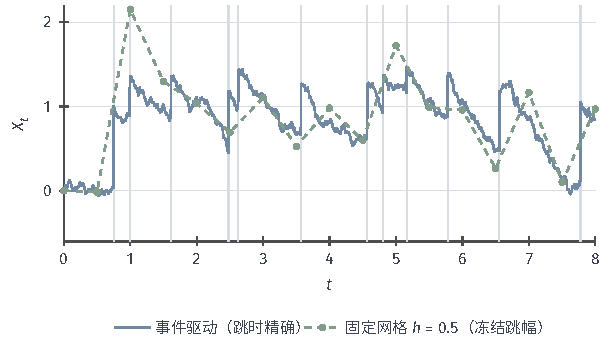
\includegraphics[width=105mm]{figures/03-optimization-evolution-and-signals/02-processes-and-trajectory-evolution/tikz/ctsp-jump-event-grid/figure.pdf}
  \caption{事件驱动与固定网格的跳跃模拟。模型$\mathrm dX=-X\,\mathrm dt+0.25\,\mathrm dW+\gamma(X_-)\,\mathrm dN$，跳幅$\gamma(x)=1-0.6x$依赖跳前状态，事件速率$\lambda=1.2$，固定随机种子。灰色竖线为事件时刻。蓝线在细网格上推进扩散，并在事件时刻精确跳跃；绿色折线用步长$h=0.5$的网格、相同的Brownian增量与每格事件数，跳幅冻结在格首状态。两者的差来自跳时错位与同一格内多次事件。}
  \label{fig:ctsp-jump-event-grid}
\end{figure}

跳跃部分与连续部分的误差来源不同，报告时应分开。精确模拟跳跃而只近似扩散时，误差分析回到上一小节；跳跃也只能近似时（例如强度没有可用的上界，或跳幅分布难以采样），应分别说明跳跃近似与连续步进各自的误差，以及两者怎样随$h$变化。

\subsection{强误差、弱误差与长期偏差}
\label{sec:ctsp-error-types}

\paragraph{两种误差}
衡量数值解的好坏，首先要说清比较的对象。若关心的是单条路径，例如要用模拟路径检验某个依赖路径细节的控制策略，就应当在同一条Brownian路径下比较真解与数值解，即用$\Delta\bm W_k=\bm W_{t_{k+1}}-\bm W_{t_k}$驱动数值格式。终点的\term{强误差}（strong error）定义为$\bigl(\mathbb E\|\bm X_T-\widehat{\bm X}_n\|_2^p\bigr)^{1/p}$，常取$p=1$或$2$。若关心的只是期望，例如某个读数的平均，就不必让两条路径配对，只比较测试函数$\varphi$的期望，定义\term{弱误差}（weak error）为$|\mathbb E\varphi(\bm X_T)-\mathbb E\varphi(\widehat{\bm X}_n)|$。

两类误差的阶数不同。在漂移与扩散全局Lipschitz、线性增长、初值平方可积，并且系数关于时间有$\frac12$阶Hölder正则的条件下，Euler--Maruyama的强误差满足
\[
  \max_{k\leq n}\bigl(\mathbb E\|\bm X_{t_k}-\widehat{\bm X}_k\|_2^2\bigr)^{1/2}\leq C_Th^{1/2},
\]
其证明与定理~\ref{thm:ctsp-sde-existence}相同：把数值解写成连续插值，相减后用Lipschitz条件、Itô等距与Doob不等式得到Grönwall型不等式，额外的$h$来自系数在一个步长内的变化。在系数与测试函数具有至四阶的有界连续导数等条件下，弱误差满足$|\mathbb E\varphi(\bm X_T)-\mathbb E\varphi(\widehat{\bm X}_n)|\leq C_{\varphi,T}h$\scite{math-kloeden1992numerical-sde}。Milstein方法把强误差提高到一阶，弱误差仍为一阶。

图~\ref{fig:ctsp-em-orders}用几何Brownian运动核对了这两个阶。强误差在双对数坐标中的斜率接近$\frac12$，弱误差的斜率接近$1$。

\begin{figure}[htbp]
  \centering
  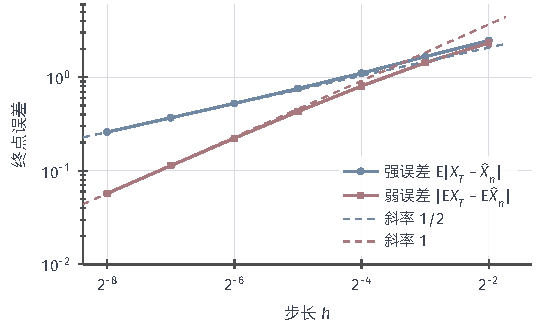
\includegraphics[width=95mm]{figures/03-optimization-evolution-and-signals/02-processes-and-trajectory-evolution/tikz/ctsp-em-orders/figure.pdf}
  \caption{Euler--Maruyama方法的终点误差，双对数刻度。模型为几何Brownian运动$\mathrm dX=2X\,\mathrm dt+X\,\mathrm dW$，$X_0=1$，$T=1$。蓝点为强误差$\mathbb E|X_T-\widehat X_n|$，由$4000$条Brownian路径（固定随机种子）在最细网格上生成增量、再合并到各粗网格，与显式解在同一路径上比较；红点为$\varphi(x)=x$的弱误差，取精确值$|e^{2}-(1+2h)^{1/h}|$。虚线是斜率$\frac12$与$1$的参考线。}
  \label{fig:ctsp-em-orders}
\end{figure}

弱误差小并不说明路径接近。设$\bm X'$是与$\bm X$独立同分布的另一份副本，则对一切可积的$\varphi$，弱误差为零，而$\mathbb E\|\bm X_T-\bm X'_T\|_2^2=2\operatorname{tr}\operatorname{Cov}(\bm X_T)$并不小。两种误差衡量的是不同的事情：强误差要求“同一噪声下走到同一个地方”，弱误差只要求“走到各处的概率一样”。

\paragraph{弱误差的望远镜机制}
弱误差为什么比强误差高阶？答案来自第~\ref{sec:ctsp-backward-forward}节的后向方程。令$u(t,\bm x)=\mathbb E[\varphi(\bm X_T)\mid\bm X_t=\bm x]$，它满足$\partial_tu+\mathcal Lu=0$、$u(T,\cdot)=\varphi$。于是
\[
  \mathbb E\varphi(\widehat{\bm X}_n)-\mathbb E\varphi(\bm X_T)=\sum_{k=0}^{n-1}\mathbb E\bigl[u(t_{k+1},\widehat{\bm X}_{k+1})-u(t_k,\widehat{\bm X}_k)\bigr],
\]
因为右端望远镜相消后剩下$\mathbb Eu(T,\widehat{\bm X}_n)-u(0,\bm X_0)$。对每一项，从$\widehat{\bm X}_k$出发，精确转移使$u$的期望保持不变；数值的一步转移与精确转移的前两阶矩只相差$O(h^2)$，在$u$有界的高阶导数下，每一项是$O(h^2)$。共$n=T/h$项，累计为$O(h)$。强误差没有这种抵消：每一步的路径误差是$O(h)$量级的随机量，其均方的累计按随机游走方式增长，得到$O(h^{1/2})$。

\paragraph{时间离散误差与Monte Carlo误差}
实际计算期望$\mathbb E\varphi(\bm X_T)$时，用$M$条独立的数值路径求平均，误差有两个来源：
\[
  \mathbb E\Bigl(\frac1M\sum_{i=1}^M\varphi(\widehat{\bm X}^{(i)}_n)-\mathbb E\varphi(\bm X_T)\Bigr)^2=\underbrace{\bigl(\mathbb E\varphi(\widehat{\bm X}_n)-\mathbb E\varphi(\bm X_T)\bigr)^2}_{\text{离散偏差}^2}+\underbrace{\frac{\operatorname{Var}\varphi(\widehat{\bm X}_n)}M}_{\text{抽样方差}} .
\]
弱一阶时偏差约为$Ch$，计算量约为$M/h$。要使均方根误差达到$\varepsilon$，需要$h\sim\varepsilon$、$M\sim\varepsilon^{-2}$，总计算量约为$\varepsilon^{-3}$。减小步长与增加路径数各自只能压低一项，应当按两项的平衡分配预算。

\paragraph{长期偏差}
上述误差界中的常数$C_T$一般随$T$增长，有限时段的收敛不能直接推出长期行为的近似：$h\to0$与$T\to\infty$两个极限不能随意交换。OU过程的例子很清楚。数值链的稳态方差$\sigma^2/[\lambda(2-\lambda h)]$与真值$\sigma^2/(2\lambda)$相差的比例为$\lambda h/(2-\lambda h)$，这个偏差不随运行时间增长而消失；步长超过$2/\lambda$时数值链甚至发散，而连续模型对任何初值都稳定。数值链的不变分布是否存在、偏离真实不变分布多少，需要单独分析。下一节用数值链做采样时，这个偏差将成为必须处理的问题。
